\section{Versuchsaufbau und Versuchsdurchführung}

\begin{flushleft}
    Der Versuchsaufbau besteht hauptsächlich aus einer transparenten Grundplatte, an welcher ein Reflektionsschirm sowie ein verschiebbarer Laser angebracht ist.
    Unter dieser Grundplatte befindet sich eine Winkelscheibe um den Laser entsprechend einzustellen.
    Zusehen ist dies in Abbildung \ref{Abbildung4}.
\end{flushleft}

\begin{figure}[H]
    \centering
    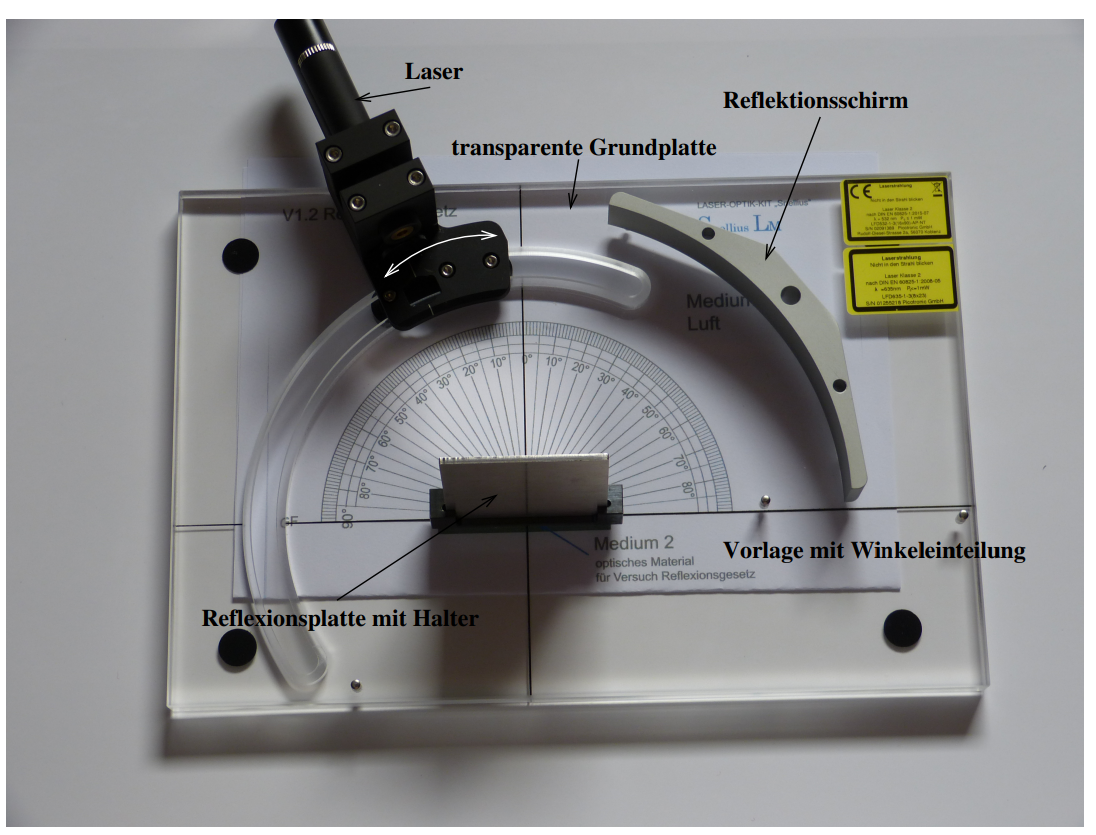
\includegraphics[height=80mm]{bilder/Ab4.png}
    \caption{Transparente Grundplatte mit Laser und Reflektionsschirm \cite{a1}.\label{Abbildung4} }
\end{figure}

\begin{flushleft}
    Der Laser besteht dabei aus zwei Strahlen.
    Der grüne Laser ist der untere und emittiert grünes Licht mit der Wellenlänge $\lambda = 532\,\unit{\nano\meter}$.
    Der rote Laser ist der obere und emittiert rotes Licht mit der Wellenlänge $\lambda = 635\,\unit{\nano\meter}$.
    In der Mitte bzw. über die Platte verteilt befinden sich kleine Halterungen für die jeweiligen Elemente.
    Verwendet werden ebenso optische Elemente die für die Überprüfung bzw. Beobachtung der optischen Phänomene wichtig sind.
    Zusehen sind diese in der Abbildung \ref{Abbildung5}
\end{flushleft}

\begin{figure}[H]
    \centering
    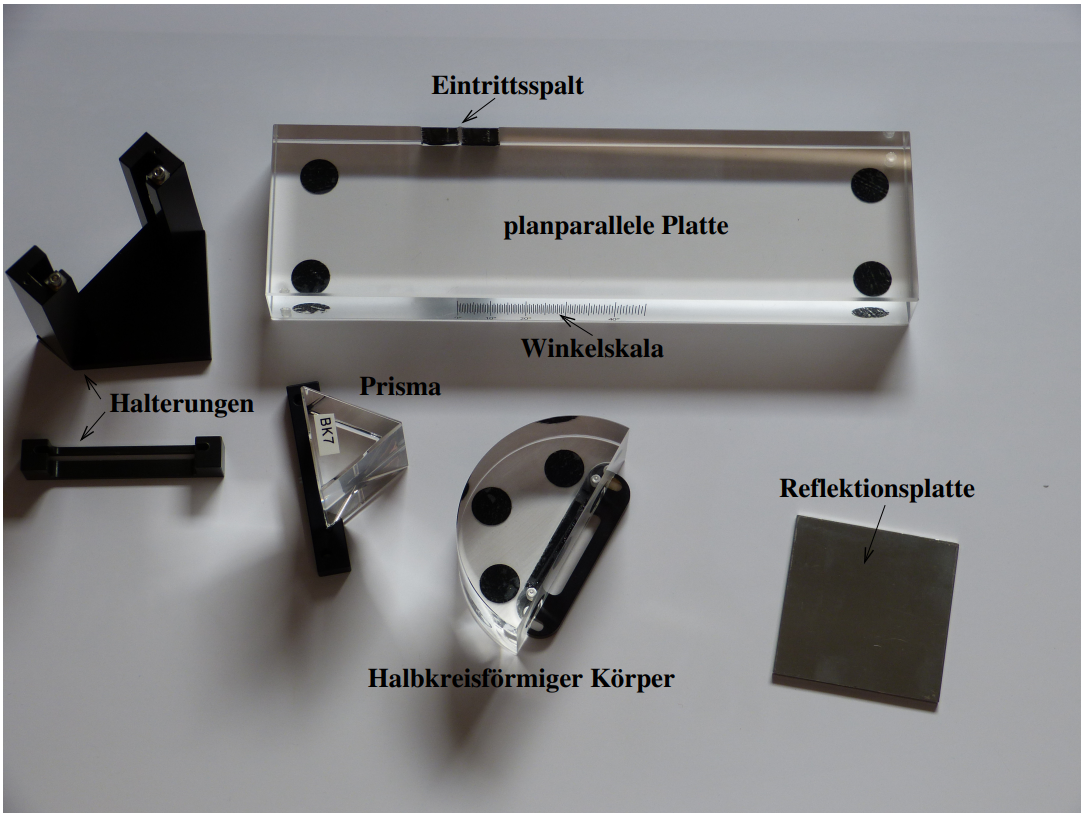
\includegraphics[height=80mm]{bilder/Ab5.png}
    \caption{Die im Versuch verwendeten optischen Elemente \cite{a1}.\label{Abbildung5} }
\end{figure}

\subsection{Reflexionsgesetz}

\begin{flushleft}
    Eine Reflektionsplatte wird in der Mitte angebracht und der grüne Laser wird benutzt.
    Danach werden für sieben verschiedenen Einfallswinkel $\alpha_{1}$ der dazugehörige Ausfallswinkel $\alpha_{2}$ abgelesen und notiert.
\end{flushleft}

\subsection{Brechungsgesetz}

\begin{flushleft}
    Als nächstes wird die Reflektionsplatte durch eine planparallele Platte ersetzt. 
    Wichtig dabei ist, dass der markierte Eintrittsspalt in Richtung des Lasers ausgerichtet ist.
    Es wird immer noch der grüne Laser verwendet.
    Im folgenden werden für sieben verschiedene Einfallswinkel $\alpha$ die dazugehörigen Brechungswinkel $\beta$ abgelesen und notiert.
\end{flushleft}

\subsection{Prisma}

\begin{flushleft}
    Nun wird die planparallele Platte durch ein Prisma und die Winkelvorlage durch eine bessere Winkelvorlage ersetzt.
    Diesmal werden beide Laser verwendet.
    Der Einfallswinkel $\alpha_{1}$ für den Laser wird für fünf verschiedene Winkel, im Bereich von $30\unit{\degree}$ bis $60\unit{\degree}$, eingestellt und die dabei entstehenden Austrittswinkel $\alpha_{2}$ gemessen.
\end{flushleft}

\subsection{Beugung am Gitter}

\begin{flushleft}
    Als letztes wird das Prisma durch ein Gitter in einer Halterung gewechselt.
    Dieses Gitter wird jedoch nicht auf der transparenten Grundplatte platziert, sondern am Rand der Platte vor dem Laser, damit beide Laserstrahlen durch das Gitter laufen.
    Danach werden für beide Laserstrahlen die Beugungsmaxima aller drei Gitter gemessen.
\end{flushleft}
